\documentclass{beamer}

% === AUTOR === (((
\author{\textit{Por Erick I. Rodríguez Juárez.}}
% )))

% === PAQUETES === (((
% \usepackage{makeidx}
% \usepackage{xltxtra}
\usepackage{amsfonts}
\usepackage{amsmath}
\usepackage{amssymb}
% \usepackage{fullpage}
\usepackage{tikz}
\usetikzlibrary{arrows.meta}
\usepackage{graphicx}
% )))

% === TIPOGRAFÍA === (((
% \setmainfont[
  % BoldFont       = bodonibi,
	% ItalicFont     = Century modern italic2.ttf,
	% BoldItalicFont = bodonibi,
	% SmallCapsFont  = lmromancaps10-regular.otf
% ]{Century_modern.ttf}
% )))

% === COMANDOS === (((
% \newcommand{\dis}{\displaystyle}
% \newcommand{\qed}{\hspace{0.5cm}\rule{0.16cm}{0.4cm}}
% \newcommand{\operator}[1]{\mathop{\vphantom{\sum}\mathchoice
% {\vcenter{\hbox{\huge $#1$}}}
% {\vcenter{\hbox{\Large $#1$}}}{#1}{#1}}\displaylimits}
% \newcommand{\suma}{\operator{
\includegraphics[scale=0.09]{FOTOS/Sigma.png}}}
% \setlength{\parindent}{0mm}
% )))

% === ITALICA EN ENTORNO MATEMÁTICO === (((
% \DeclareSymbolFont{italics}{\encodingdefault}{\rmdefault}{m}{it}
% \DeclareSymbolFontAlphabet{\mathit}{italics}
% \ExplSyntaxOn
% \int_step_inline:nnnn { `A } { 1 } { `Z }
 % {  \exp_args:Nf \DeclareMathSymbol{\char_generate:nn{#1}{11}}{\mathalpha}{italics}{#1} }
% \int_step_inline:nnnn { `a } { 1 } { `z } {  \exp_args:Nf \DeclareMathSymbol{\char_generate:nn{#1}{11}}{\mathalpha}{italics}{#1}}
% \ExplSyntaxOff
% )))

\begin{document}

\frame{\titlepage}

\begin{frame}[t]
	\frametitle{Problemas de Valor Inicial.}
	\begin{block}{}
		En esta unidad estudiaremos las ecuaciones diferenciales lineales de orden \(n\) (\(n>1\)) las cuales tienen la siguiente forma:
		\begin{equation}
			a_n(x) y^{(n)} + \;\cdots\; + a_1(x) y' +a_0(x) y=g(x).
			\label{eq:definicion_lineal}
		\end{equation}
		donde \(a_n, \;\ldots,\; a_1,a_0,g\), son funciones de valores real en un intervalo \(I\).
	\end{block} \vspace{5mm}
	\begin{block}{Problema de Valor Inicial}
		\textbf{Definición.} Un \textbf{P.V.I. de orden \(n\)} consiste en resolve la ecuación diferncial (\ref{eq:definicion_lineal}) sujeta a las condiciones
		\[
			y(x_0) = y_0, \;\cdots\; y^{(n-1)} (x_0) = y_{n-1}.
		\]
		donde: \(y_0,y_1, \;\cdots\; y_{n-1}\) son constante reales dadas.
	\end{block}
\end{frame}

\begin{frame}[t]
	\begin{block}{}
		\textbf{Interpretación geométrica:} P.V.I. de \(2^{do}\) Orden.
		\[
			\begin{array}{rcl}
				a_2(x) y'' +a_1(x) y' +a_0(x) y & = & g(x) \\[2mm]
				y(x_0) = y_0 , \hspace{5mm} y' (x_0) & = & y_1 >0.
			\end{array}
		\]
		\begin{figure}[ht]
			\centering
			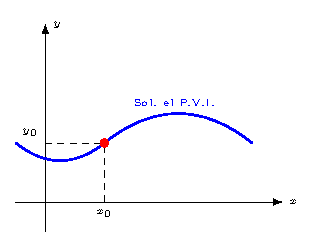
\includegraphics[width= 0.6 \linewidth]{IMAGENES/1/tikz.pdf}
		\end{figure}
	\end{block}
\end{frame}

\begin{frame}[t]
	\begin{block}{}
		\textbf{Interprteación geométrica:} P.V.I. de \(3^{er}\) Orden.
		\[
			\begin{array}{rcl}
				3y''' +5y'' -y' +7y & = & 0 \\[2mm]
				y(1) =0 \hspace{5mm} y'(1) =0 m y'' (1) & = & 0 \\[2mm]
			\end{array}
		\]
		\begin{figure}[ht]
			\centering
			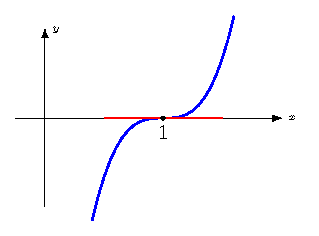
\includegraphics[width= 0.7 \linewidth]{IMAGENES/2/tikz.pdf}
		\end{figure}
	\end{block}
\end{frame}

\begin{frame}[t]
	\frametitle{Problemas de Valor en la Frontera.}
	\begin{block}{Problema de Valor en la Frontera.}
		Un \textbf{P.V.F. de orden \(n\)} consiste en resolver la ecuación diferencial (\ref{eq:definicion_lineal}) sujeto a condiciones sobre la variable dependiente \(y\) (o sus derivadas) en puntos distintos de la variable independiente, esto es
		\[
			y(x_0) =y_0 \;,\;  y(x_1) =y_1 \;, \;\ldots,\; y(x_{n-1}) =y_{n-1}. \vspace{-2.5mm}
		\]
		donde \(x_0,x_1, \;\ldots,\; x_{n-1} \in I\), y \(y_0,y_1, \;\ldots,\; y_{n-1}\) son constantes dadas.\\[-5.5mm]
		\begin{minipage}{0.3\linewidth}
			En este caso, se busca una solución de la E.D. que pase por los puntos \((x_0,y_0) , (x_1,y_1) , \;\ldots,\)\\\( (x_n,y_n)\).
		\end{minipage} \hspace{5mm}
		\begin{minipage}{0.6\linewidth}
			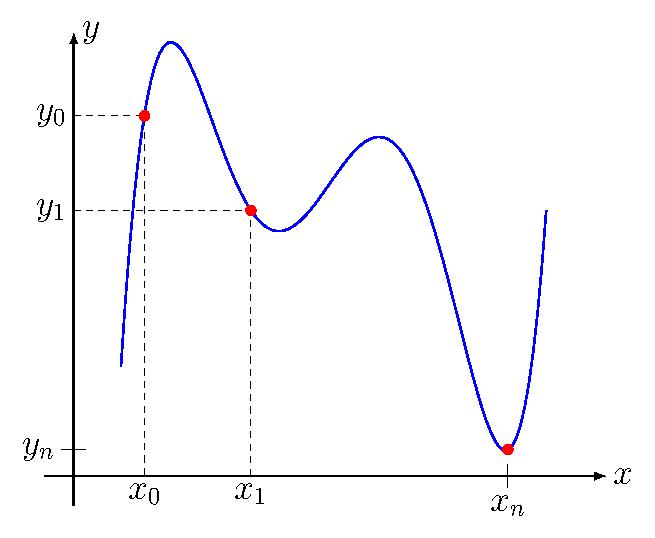
\includegraphics[width= 0.9\linewidth]{IMAGENES/3/tikz.pdf}
		\end{minipage}
	\end{block}
\end{frame}

\begin{frame}[t]
	\begin{block}{}
	\textbf{Interpretación geométrica:} P.V.F. de \(2^{do}\) Orden.
	\[
		\begin{array}{rcl}
			a_2(x) y'' +a_1(x) y' + a_0(x) y & = & g(x) \\[2mm]
			y(x_0) = y_0 , \hspace{4mm} y(x_1) & = & y_1. \vspace{-1cm}
		\end{array}
	\]
		\begin{figure}[ht]
			\centering
			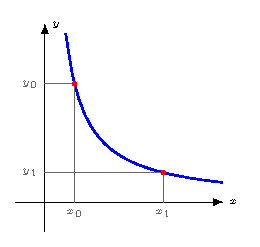
\includegraphics[width= 0.55 \linewidth]{IMAGENES/4/tikz.pdf}
		\end{figure}
	\end{block}
\end{frame}

\begin{frame}[t]
	\begin{block}{}
		Otro tipo de condiciones de frontera son:\\
		\begin{minipage}{0.3\linewidth}
			\begin{enumerate}
					\footnotesize 
				\item \(y(x_0) =y_0\), \(y' (x_1) =y_1 < 0.\)
				\item \(y'(x_0)=y_0\), \(y(x_1) =y_1\).
				\item \(y' (x_0) =y_0\), \(y'(x_0) =y_1 >0\).
			\end{enumerate}
		\end{minipage}\hspace{5mm}
		\begin{minipage}{0.6\linewidth}
			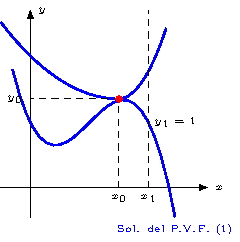
\includegraphics[width= \linewidth]{IMAGENES/5/tikz.pdf}
		\end{minipage}
	\end{block}
\end{frame}

\end{document}
